% gm-14-vectors.tex

\documentclass[xcolor=dvipsnames]{beamer}

\usepackage{cancel}
\renewcommand{\CancelColor}{\color{red}}
\usepackage{graphicx}
\usepackage{wrapfig}
\usepackage{colortbl}
\usepackage{color}
\usepackage{alltt}
\renewcommand*{\thefootnote}{\fnsymbol{footnote}}
\definecolor{myblue}{rgb}{0.8,0.85,1}

\mode<presentation>
{
  \usetheme{Warsaw}
  \setbeamercovered{transparent}
}
% \usecolortheme[named=OliveGreen]{structure}
\setbeamertemplate{navigation symbols}{} 
\setbeamertemplate{blocks}[rounded][shadow=true] 

% this is for overlaying math symbols, see https://tex.stackexchange.com/questions/12895/overlay-symbol-with-another
\def\qeq{\mathrel{%
    \mathchoice{\QEQ}{\QEQ}{\scriptsize\QEQ}{\tiny\QEQ}%
}}
\def\QEQ{{%
    \setbox0\hbox{$\longrightarrow$}%
    \rlap{\hbox to \wd0{\hss/\hss}}\box0
  }}

\newcounter{expls}
\setcounter{expls}{0}
\newcommand{\beispiel}[1]{\refstepcounter{expls}\textbf{Example \arabic{expls}: #1.}}

\newcounter{exercise}
\setcounter{exercise}{0}
\newcommand{\ubung}[0]{\refstepcounter{exercise}\textbf{Exercise \arabic{exercise}: }}

\newif\ifBCITCourse
\BCITCoursetrue
% \BCITCoursefalse
\newif\ifWhichCourse
\WhichCoursetrue
\WhichCoursefalse
\ifBCITCourse
\ifWhichCourse
\newcommand{\CourseName}{Technical Mathematics for Food Technology}
\newcommand{\CourseNumber}{MATH 1441}
\newcommand{\CourseInst}{BCIT}
\else
\newcommand{\CourseName}{Technical Mathematics for Geomatics}
\newcommand{\CourseNumber}{MATH 1511}
\newcommand{\CourseInst}{BCIT}
\fi
\else
\newcommand{\CourseName}{Philosophy and Literature}
\newcommand{\CourseNumber}{PHIL 375}
\newcommand{\CourseInst}{UBC}
\fi

\title{Vectors}
\subtitle{{\CourseNumber}, BCIT}

\author{\CourseName}

\date{November 13, 2017}

\begin{document}

\begin{frame}
  \titlepage
\end{frame}

\begin{frame}
  \frametitle{Vectors}
A vector is a special type of matrix: it has only one row or only one
column. Here are two examples of a vector,
\begin{equation}
  \label{eq:aesaimae}
  a=\left(
    \begin{array}{c}
      -2  \\
      3
    \end{array}\right)\mbox{ and }b=\left(
    \begin{array}{c}
      \frac{1}{2} \\
      7
    \end{array}\right)
\end{equation}
We add them as we would add matrices,
\begin{equation}
  \label{eq:baidohdi}
  a+b=\left(
    \begin{array}{c}
      -2 \\
      3
    \end{array}\right)+\left(
    \begin{array}{c}
      \frac{1}{2} \\
      7
    \end{array}\right)=\left(
    \begin{array}{c}
      -1.5 \\
      10
    \end{array}\right)
\end{equation}
  \begin{figure}[h]
    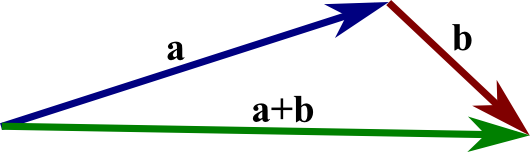
\includegraphics[scale=1]{./vector_a_plus_b.png}
  \end{figure}
\end{frame}

\begin{frame}
  \frametitle{Vector Subtraction}
We define the additive inverse $-a$ of a vector $a$ to be the vector
whose components are the additive inverses of $a$'s components.
\begin{equation}
  \label{eq:yaivujoh}
  -a=\left(
    \begin{array}{c}
      2 \\
      -3
    \end{array}\right)
\end{equation}
Vector subtraction is defined as follows: $a-b=a+(-b)$. 
\begin{equation}
  \label{eq:ahkeizoh}
  a-b=\left(
    \begin{array}{c}
      -2 \\
      3
    \end{array}\right)+\left(
    \begin{array}{c}
      -\frac{1}{2} \\
      -7
    \end{array}\right)=\left(
    \begin{array}{c}
      -2.5 \\
      -4
    \end{array}\right)
\end{equation}
  \begin{figure}[h]
    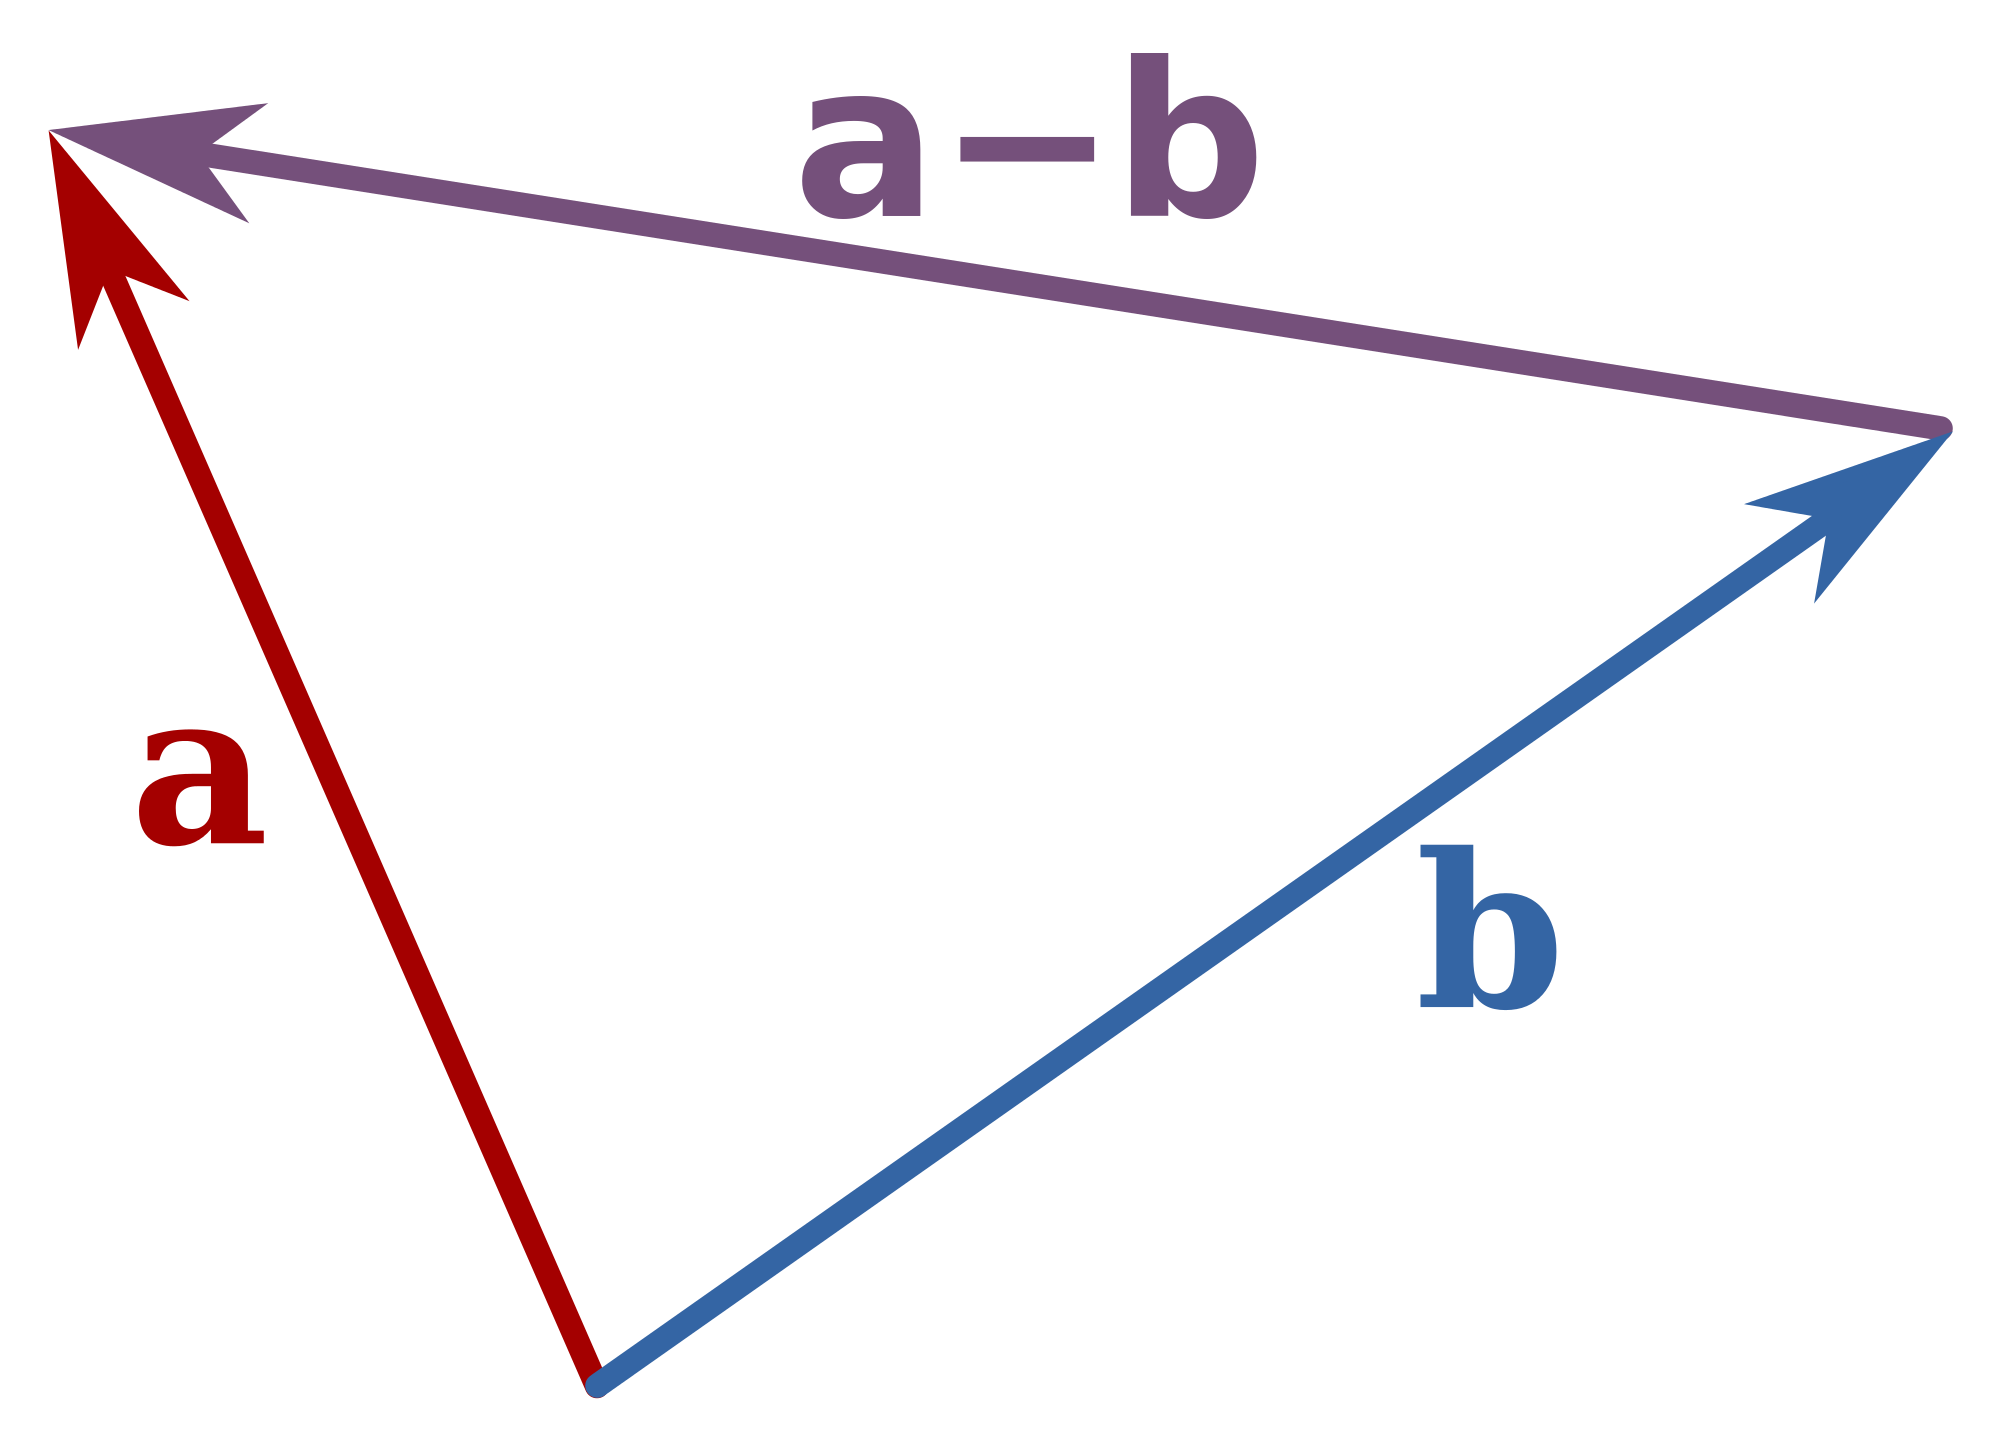
\includegraphics[scale=.07]{./vectorminus.png}
  \end{figure}
\end{frame}

\begin{frame}
  \frametitle{Scalar Multiplication}
Scalar multiplication is defined for vectors as it was for matrices. A
real number $C$ and a vector $a$ can be multiplied as follows,
\begin{equation}
  \label{eq:oyeizaeb}
  C\cdot{}a=C\cdot\left(
    \begin{array}{c}
      a_{1} \\
      a_{2}
    \end{array}\right)=
\left(
    \begin{array}{c}
      C\cdot{}a_{1} \\
      C\cdot{}a_{2}
    \end{array}\right)
\end{equation}
  \begin{figure}[h]
    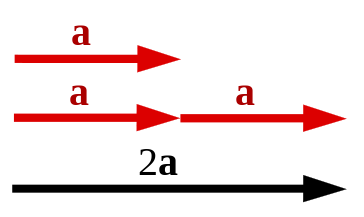
\includegraphics[scale=.5]{./scalarmultiplication.png}
  \end{figure}
\end{frame}

\begin{frame}
  \frametitle{Vectors and Geometry}
One way to interpret two-dimensional vectors is to have them describe
movement in the plane. They have no home in the coordinate system, but
only describe how to get from one point to another. By convention,
unless we have reason to do otherwise, we let them start at the origin.
  \begin{figure}[h]
    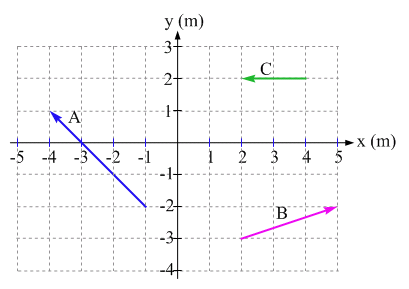
\includegraphics[scale=.5]{./veccoor.png}
  \end{figure}
\end{frame}

\begin{frame}
  \frametitle{Vectors and Angles}
Each vector (except the vector whose components are all zero) has an
angle associated with it, which mathematicians conventionally measure
counter-clockwise from the $x$-axis. You are welcome to represent the
angle any way you like as long as it is clear what you mean.
  \begin{figure}[h]
    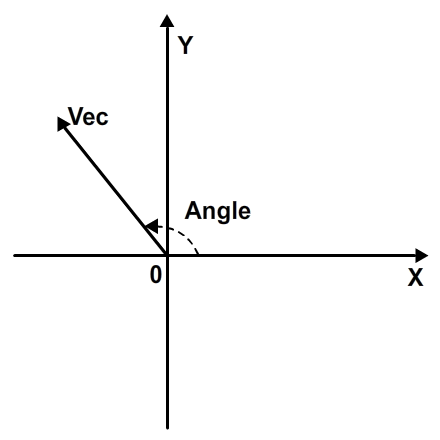
\includegraphics[scale=.5]{./AngleCartesian.png}
  \end{figure}
\end{frame}

\begin{frame}
  \frametitle{Example}
Let
\begin{equation}
  \label{eq:cieteang}
  a=\left(
    \begin{array}{c}
      -2 \\
      3
    \end{array}\right)
\end{equation}
Then
\begin{equation}
  \label{eq:rujiwath}
  \tan\alpha'=\frac{3}{-2}\longrightarrow\alpha'=-56.31^{\circ}
\end{equation}
This is not the correct angle, however. The correct angle is
$\alpha=180^{\circ}+\alpha'=123.69^{\circ}$. You can also represent it
as N$33.69^{\circ}$W. The length of the vector is
\begin{equation}
  \label{eq:kootahpa}
  |a|=\sqrt{(-2)^{2}+3^{2}}\approx{}3.61
\end{equation}
\end{frame}

\begin{frame}
  \frametitle{Exercises}
{\ubung} Calculate the length $|a_{i}|$ and the angle $\alpha_{i}$ for the following
vectors,
\begin{equation}
  \label{eq:aozurohp}
  a_{1}=\left(
    \begin{array}{c}
      7 \\
      3
    \end{array}\right)
\end{equation}
\begin{equation}
  \label{eq:atheimah}
  a_{2}=\left(
    \begin{array}{c}
      -6 \\
      -11
    \end{array}\right)
\end{equation}
\begin{equation}
  \label{eq:chefoobo}
  a_{3}=\left(
    \begin{array}{c}
      -\pi \\
      10.5
    \end{array}\right)
\end{equation}
\begin{equation}
  \label{eq:aevebuaf}
  a_{4}=\left(
    \begin{array}{c}
      \frac{7}{13} \\
      -\frac{1}{5}
    \end{array}\right)
\end{equation}
\end{frame}

\begin{frame}
  \frametitle{Vectors and Points}
{\ubung}  Jim starts at $P=(-34,19)$ (units are metres) and walks 60 metres
  on a bearing of N$79^{\circ}$E. Which vector describes Jim's
  movement? What are the coordinates of Jim's destination?
\end{frame}

\begin{frame}
  \frametitle{Vectors and Points}
  The vector $\vec{PQ}$ displaces $P$ to $Q$. The coordinates of point
  $P$ and the elements of vector $\vec{OP}$ match. To find the
  coordinates of Jim's destination in the problem on the last slide,
  note that
  \begin{equation}
    \label{eq:mohquaes}
    \vec{OQ}=\vec{OP}+\vec{PQ}
  \end{equation}
We can easily calculate the RHS (right-hand side), and the LHS provides
us with the coordinates of point $Q$.
  \begin{figure}[h]
    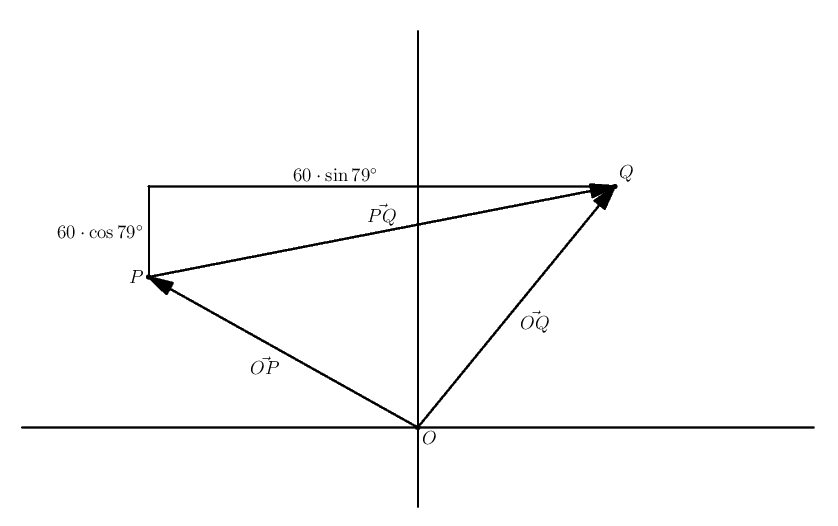
\includegraphics[scale=.3]{./vectora.png}
  \end{figure}
\end{frame}

\begin{frame}
  \frametitle{Vectors and Points}
{\ubung}  Mr.\ X walks 5km east and 2km north from $A$ to $B$. Ms.\ Y walks
  6km west and 6km north from $A$ to $C$. What angles could they have
  chosen to minimize the distance to their destination? What would be
  that minimal distance? What angle does Ms.\ Y need to choose and how
  far does she need to walk if she wants to rejoin Mr.\ X, going from
  $C$ to $B$?
\end{frame}

\begin{frame}
  \frametitle{Vectors and Points}
For the problem on the last slide, we are interested in the vector
$\vec{CB}$. Note that
\begin{equation}
  \label{eq:iethaozo}
  \vec{CB}=\vec{CO}+\vec{OB}=\vec{OB}-\vec{OC}
\end{equation}
The solutions are
\begin{equation}
  \label{eq:theelihe}
  \begin{array}{rcccl}
    |\vec{OB}| & = & \sqrt{5^{2}+2^{2}} & \approx & 5.39 \\
    |\vec{OC}| & = & \sqrt{6^{2}+6^{2}} & \approx & 8.49 \\
    |\vec{CB}| & = & \sqrt{11^{2}+(-4)^{2}} & \approx & 11.70 \\
    \arctan\frac{2}{5} & \approx & 21.80^{\circ} & & \mbox{bearing}\approx{}N68.20^{\circ}E \\
    \arctan\frac{6}{6} & = & 45^{\circ} & & \mbox{bearing}=N45^{\circ}W \\
    \arctan\frac{4}{11} & \approx & 19.98^{\circ} & & \mbox{bearing}\approx{}S70.02^{\circ}E \\
  \end{array}
\end{equation}
\end{frame}

\begin{frame}
  \frametitle{Area: Triangle}
  Consider the following triangle:
  \begin{figure}[h]
    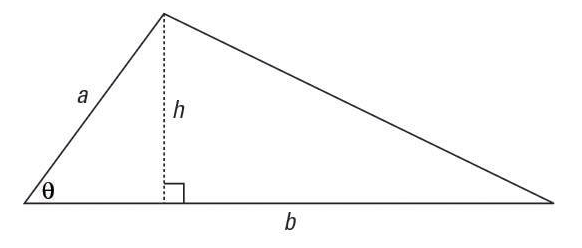
\includegraphics[scale=.5]{./areatri.png}
  \end{figure}
  Start with the traditional formula for the area of this triangle,
  \begin{equation}
    \label{eq:oquehota}
    A=\frac{1}{2}bh
  \end{equation}
\end{frame}

\begin{frame}
  \frametitle{Area: Triangle}
  \begin{figure}[h]
    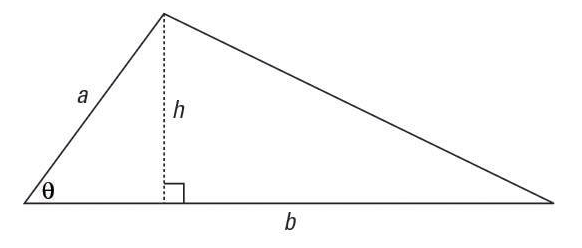
\includegraphics[scale=.5]{./areatri.png}
  \end{figure}
  Then look at the smaller triangle to the left. Because the height is
  drawn perpendicular to the base, the sides and height form a right
  triangle. The acute angle $\theta$ has a sine equivalent to the
  following:
  \begin{equation}
    \label{eq:ayooshoh}
    \sin\theta=\frac{\mbox{opposite}}{\mbox{hypotenuse}}=\frac{h}{a}
  \end{equation}
\end{frame}

\begin{frame}
  \frametitle{Area: Triangle}
  \begin{figure}[h]
    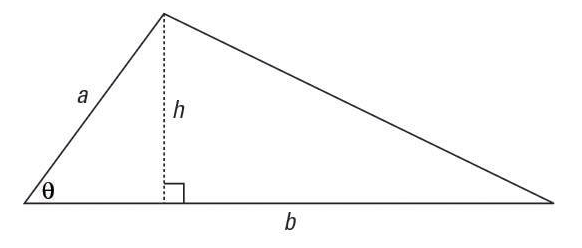
\includegraphics[scale=.5]{./areatri.png}
  \end{figure}
If you solve that equation for $h$ by multiplying each side by $a$,
you get
\begin{equation}
  \label{eq:gohgaese}
  \sin\theta=\frac{h}{a}
\end{equation}
\begin{equation}
  \label{eq:sheichuc}
  a\sin\theta=h
\end{equation}
\end{frame}

\begin{frame}
  \frametitle{Area: Triangle}
  \begin{figure}[h]
    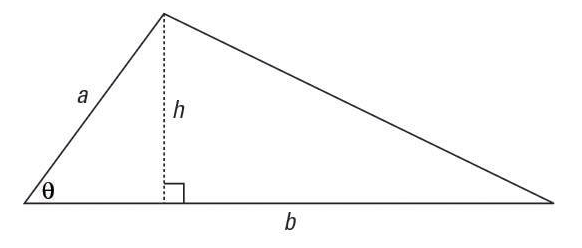
\includegraphics[scale=.5]{./areatri.png}
  \end{figure}
  Replace the $h$ in the traditional formula with its equivalent from
  the preceding equation, and you get
  \begin{equation}
    \label{eq:eakohcel}
    A=\frac{1}{2}bh=\frac{1}{2}b(a\sin\theta)=\frac{1}{2}ab\sin\theta
  \end{equation}
\end{frame}

\begin{frame}
  \frametitle{Area: Triangle}
  Two linearly independent vectors correspond to a triangle. Two
  vectors $a$ and $b$ are \alert{linearly dependent} if and only if
  $a=C\cdot{}b$ for a real number $C$. The cross product $a\times{}b$
  is the vector which is perpendicular to both $a$ and $b$, follows
  the right-hand rule, and whose length is the area of the
  parallelogram generated by $a$ and $b$. Knowing $a$ and $b$, how
  would you calculate $|a\times{}b|$?
  \begin{figure}[h]
    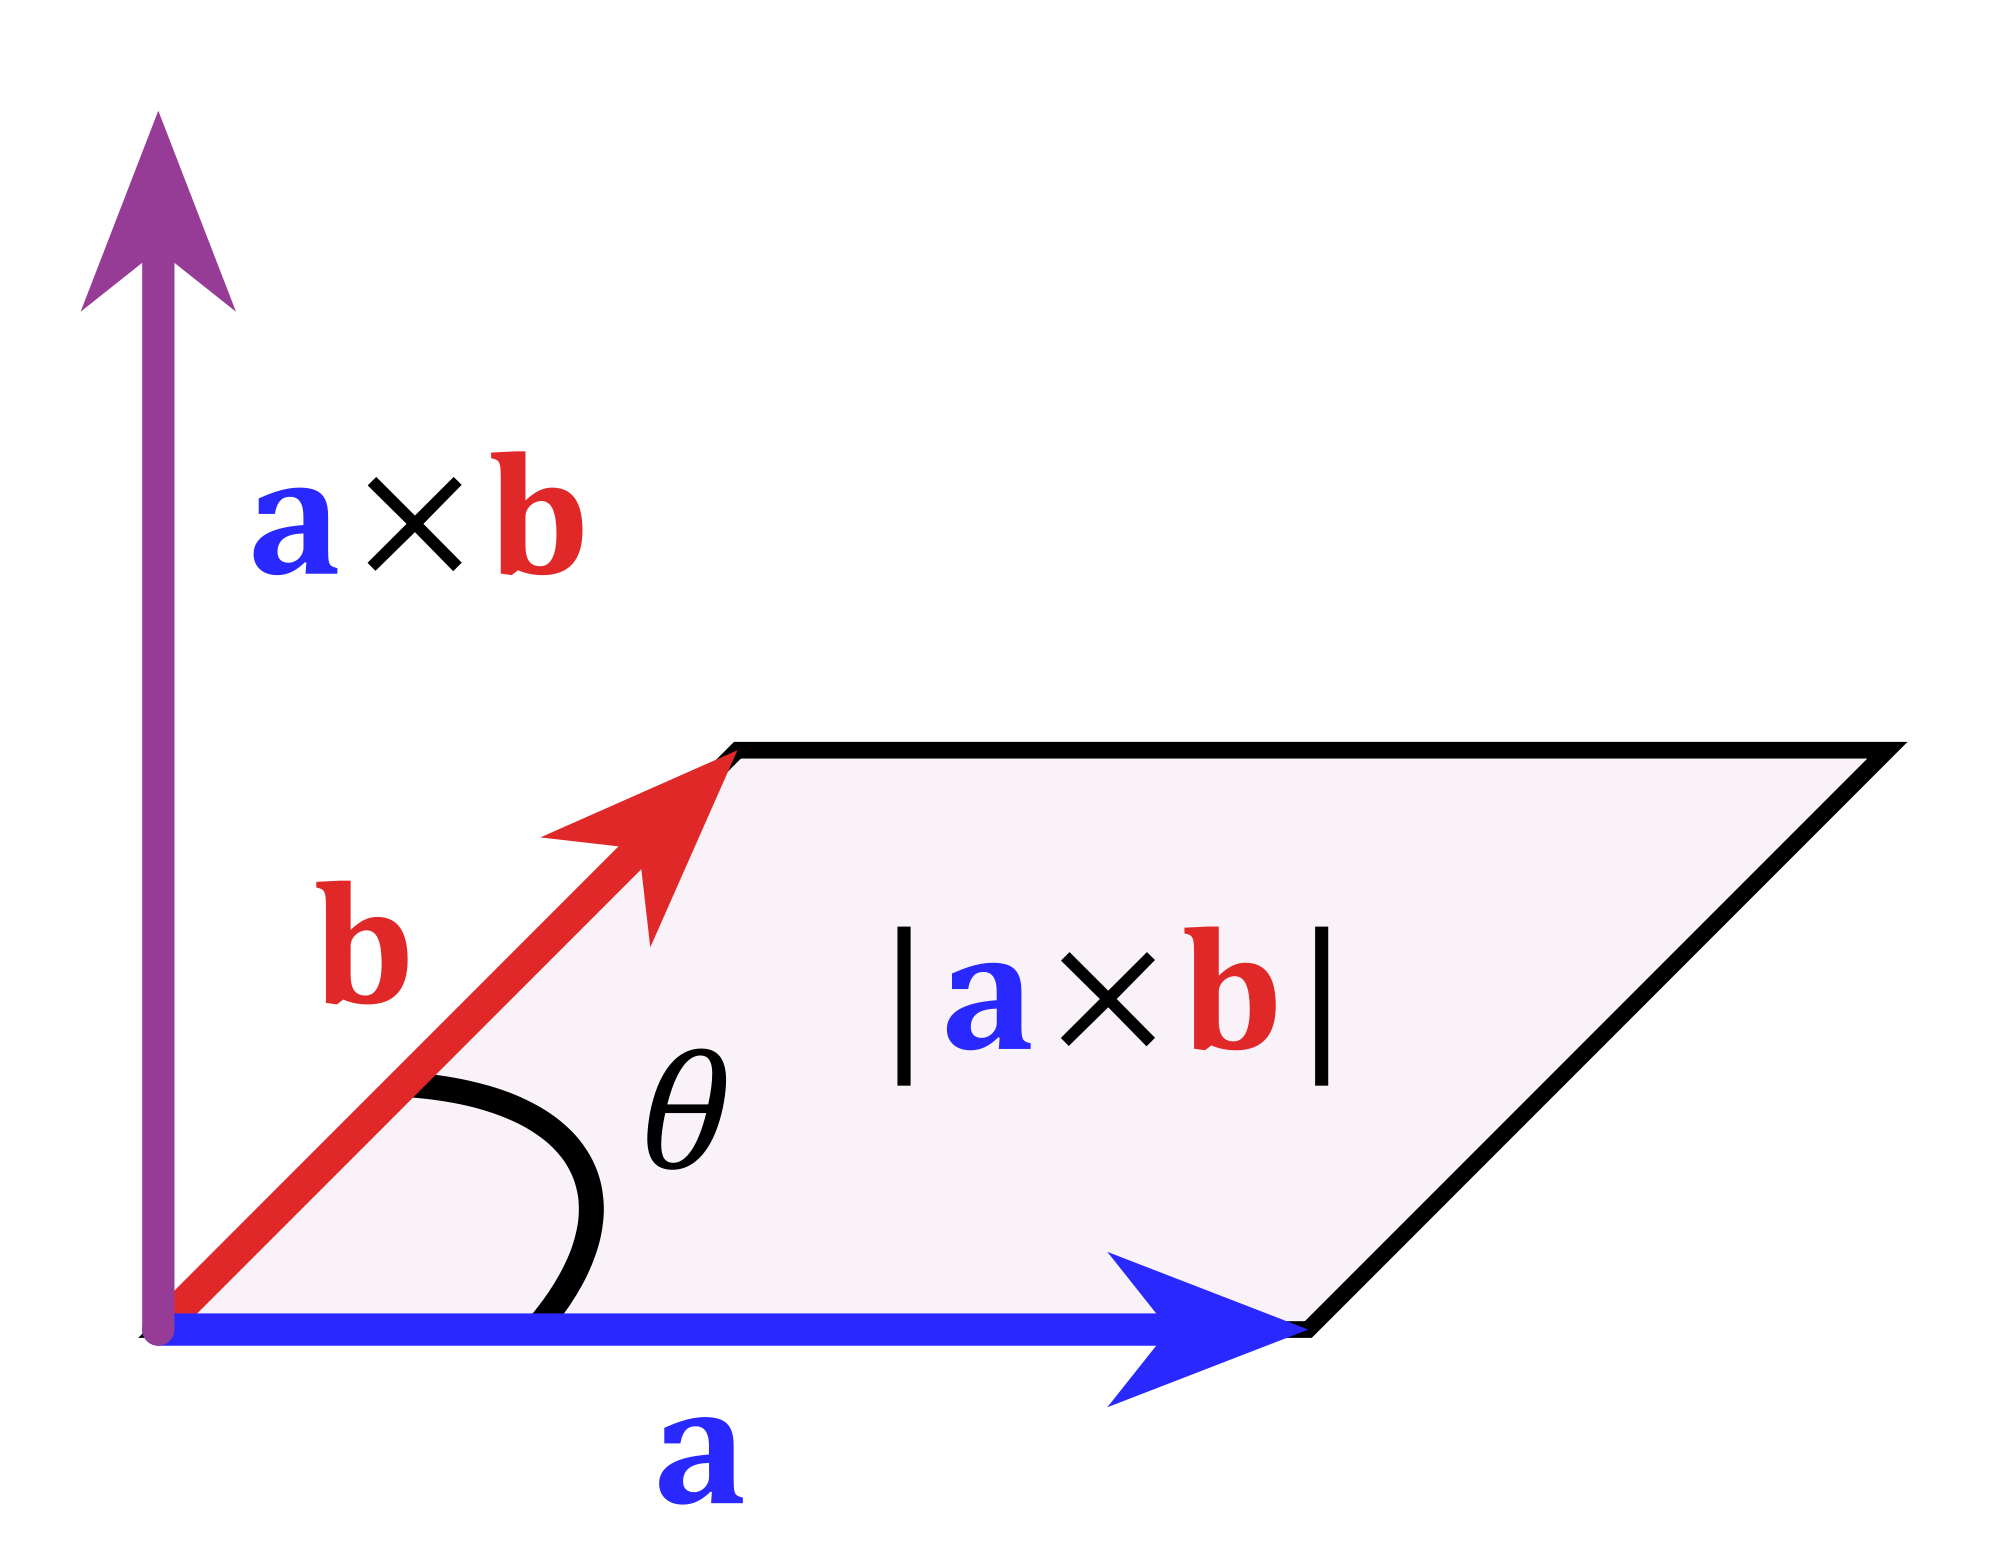
\includegraphics[scale=.08]{./Gyvro.png}
  \end{figure}
\end{frame}

\begin{frame}
  \frametitle{Area: Triangle}
The length of the cross product is
\begin{equation}
  \label{eq:xoociegh}
|a\times{}b|=|a|\cdot{}|b|\cdot\sin\theta
\end{equation}
where $\theta$ is the angle between $a$ and $b$.
  \begin{figure}[h]
    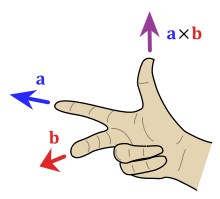
\includegraphics[scale=.7]{./right_hand_rule_cross_product.png}
  \end{figure}
\end{frame}

\begin{frame}
  \frametitle{Area: Triangle Exercises}
{\ubung} Find the area for the triangle generated by 
\begin{equation}
  \label{eq:aateeyop}
a=\left(
  \begin{array}{c}
    4 \\
    3
  \end{array}\right)\mbox{ and }
b=\left(
  \begin{array}{c}
    7 \\
    -1
  \end{array}\right)
\end{equation}
{\ubung} Find the area for the parallelogram generated by 
\begin{equation}
  \label{eq:deighooz}
a=\left(
  \begin{array}{c}
    -301 \\
    754
  \end{array}\right)\mbox{ and }
b=\left(
  \begin{array}{c}
    590 \\
    -538
  \end{array}\right)
\end{equation}
\end{frame}

\begin{frame}
  \frametitle{Area: Trapezoid}
{\ubung} Find the formula for the area of a trapezoid.
  \begin{figure}[h]
    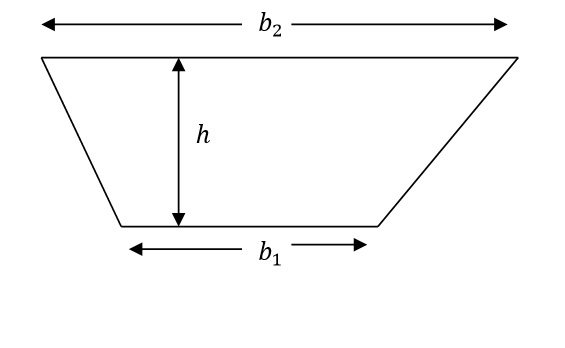
\includegraphics[scale=.5]{./trapezoid.png}
  \end{figure}
\end{frame}

\begin{frame}
  \frametitle{Area: Units}
Two common units of area are the \alert{hectare} (ha) and the \alert{acre}.
\begin{equation}
  \label{eq:ohfohdae}
1\mbox{ha}=100\mbox{m}\cdot{}100\mbox{m}
\end{equation}
\begin{equation}
  \label{eq:eicohrei}
1\mbox{acre}=43560\mbox{ft}^2
\end{equation}
Note that $1$ft$=0.3048$m. Historically, an acre was the amount of
land one man with one ox could plow in one day.
\end{frame}

\begin{frame}
  \frametitle{Vector Resultant}
{\ubung}  An office safe was lowered from an office building by two cables
  attached to buildings on opposite sides of the street. At one time
  the cables formed angles of $42^{\circ}$ and $76^{\circ}$ with the
  buildings. Find the pull on each of the cables if the safe weighed
  1250 pounds.
  \begin{figure}[h]
    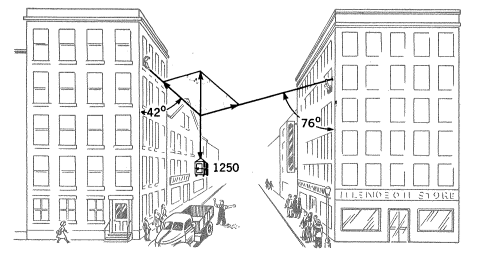
\includegraphics[scale=.55]{./vector-resultant-01.png}
  \end{figure}
\end{frame}

\begin{frame}
  \frametitle{Vector Resultant Exercise}
  {\ubung} Two ropes hold a 175 Newton crate as shown in the figure.
  Find the tensions $T_{1}$ and $T_{2}$ in the ropes. (Hint: move the
  vectors so that they are tail to head to form a triangle. The vector
  sum $T_{1}+T_{2}$ must equal 175 Newton for equilibrium.)
  \begin{figure}[h]
    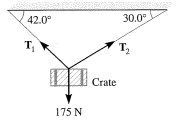
\includegraphics[scale=1]{./tri-24.png}
  \end{figure}
\end{frame}

\begin{frame}
  \frametitle{Vector Resultant Exercise}
  {\ubung} Find the tension $T$ in the left guy wire attached to the
  top of the tower as shown in the figure. (Hint: the horizontal
  component of the tensions must be equal and opposite for
  equilibrium. Thus, move the tension vectors tail to head to form a
  triangle with a vertical resultant. This resultant equals the upward
  force at the top of the tower for equilibrium. This last force is
  not shown and does not have to be calculated.)
  \begin{figure}[h]
    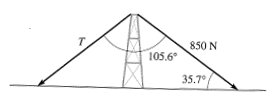
\includegraphics[scale=1]{./tri-17.png}
  \end{figure}
\end{frame}

\begin{frame}
  \frametitle{Area: Acre}
  \begin{figure}[h]
    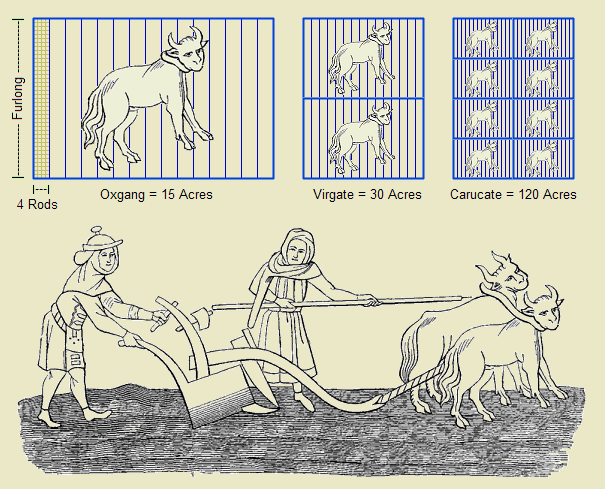
\includegraphics[scale=.45]{./acre.png}
  \end{figure}
\end{frame}

\begin{frame}
  \frametitle{Area: Units Exercises}
{\ubung} Find the answer as a complete sentence.
  \begin{enumerate}
  \item A plot has an area of 68 acres. Determine the area in
    hectares.
  \item A quarter section of land is one quarter of a mile by mile
    plot. Determine the area of a quarter section.
    \begin{enumerate}[a]
    \item Expressed in acres (recall that \mbox{1 mile}$=1760$ yards
      and \mbox{1 yard}$=3$ feet).
    \item Expressed in hectares.
    \end{enumerate}
  \end{enumerate}
\end{frame}

\begin{frame}
  \frametitle{Volume: Cone}
Consider a frustum. 
  \begin{figure}[h]
    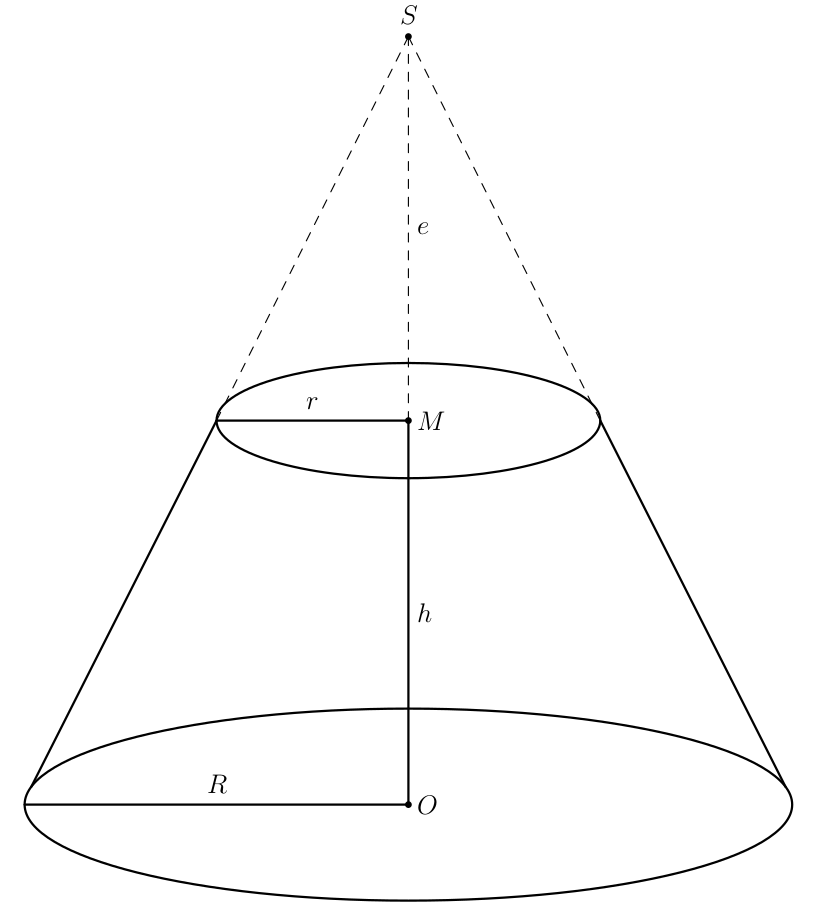
\includegraphics[scale=.22]{./frustum.png}
  \end{figure}
\end{frame}

\begin{frame}
  \frametitle{Volume: Cone}
  First off, verify that
  \begin{equation}
    \label{eq:oeveezee}
    (a-b)^{3}=(a^{2}+ab+b^{2})(a-b)
  \end{equation}
Let $A$ be the base area of the frustum and $a$ the base area of the
cone on top of the frustum. Let $\alpha$ be the angle between the
revolution axis of the cone and the generating side. Then
\begin{equation}
  \label{eq:aroowiej}
  \frac{\sqrt{a}}{e}=\frac{\sqrt{r^{2}\pi}}{e}=\frac{r\sqrt{\pi}}{e}=\sqrt{\pi}\tan\alpha=\frac{R\sqrt{\pi}}{e+h}=\notag
\end{equation}
\begin{equation}
  \label{eq:hopeexee}
  \frac{\sqrt{R^{2}\pi}}{e+h}=\frac{\sqrt{A}}{e+h}
\end{equation}
\end{frame}

\begin{frame}
  \frametitle{Volume: Cone}
  (\ref{eq:hopeexee}) gives us
  \begin{equation}
    \label{eq:iegaiqua}
    e=h\cdot\frac{\sqrt{a}}{\sqrt{A}-\sqrt{a}}
  \end{equation}
  and
  \begin{equation}
    \label{eq:eoqueeci}
    e+h=h\cdot\frac{\sqrt{A}}{\sqrt{A}-\sqrt{a}}
  \end{equation}
Now we make an assumption that we leave to intuition for
justification: the ratio of the volumes of a cone and a cylinder with
the same dimensions (radius and height) is constant, i.e.
\begin{equation}
  \label{eq:aixiiyee}
  V_{\mbox{cone}}=c\cdot{}V_{\mbox{cylinder}}
\end{equation}
As we know the formula for the volume of a cylinder (base times
height), finding $c$ will give us the formula for the cone.
  \end{frame}

\begin{frame}
  \frametitle{Volume: Cone}
  The volume of the frustum is
  \begin{equation}
    \label{eq:ailaecho}
  V_{\mbox{frustum}}=cA(e+h)-cae
  \end{equation}
  Use (\ref{eq:oeveezee}), (\ref{eq:iegaiqua}) and (\ref{eq:eoqueeci})
  for the following equation,
\begin{equation}
  \label{eq:ohchoomu}
  V_{\mbox{frustum}}=c(A+\sqrt{Aa}+a)h
\end{equation}
Now consider what happens as $a$ tends to $A$. The frustum becomes a cylinder,
and we find that
\begin{equation}
  \label{eq:uuchiroo}
  V=3cAh
\end{equation}
But we know that, for a cylinder, $V=Ah$, so $c=1/3$, and we conclude
that the volume of a cone is
\begin{equation}
  \label{eq:wutaecah}
  V_{\mbox{cone}}=\frac{1}{3}r^{2}\pi{}h
\end{equation}
\end{frame}

\begin{frame}
  \frametitle{Volume: Pyramid}
  Let the pyramid have the following dimensions: $a$ (side), $b$
  (side), $h$ (height).

\bigskip

Again, we make the assumption that the ratio of the volumes of
pyramids and rectangular cuboids (the right rectangular prism that
looks like a cube except that all the side lengths may be different)
are constant if the dimensions are the same, i.e.
\begin{equation}
  \label{eq:aetoowek}
  c\cdot{}V_{\mbox{cuboid}}=c\cdot{}a\cdot{}b\cdot{}h=V_{\mbox{pyramid}}
\end{equation}
\end{frame}

\begin{frame}
  \frametitle{Volume: Pyramid}
Now consider a cube, where all the sides are the same. It can be
divided up into 6 pyramids, whose tops are at the centre of the cube.
  \begin{figure}[h]
    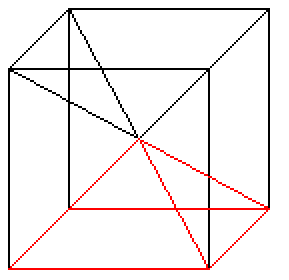
\includegraphics[scale=.5]{./pyramid08.png}
  \end{figure}
\end{frame}

\begin{frame}
  \frametitle{Volume: Pyramid}
  It follows that
  \begin{equation}
    \label{eq:jeisaure}
    c=\frac{\frac{1}{6}a^{3}}{a^{2}\cdot{}\frac{a}{2}}=\frac{1}{3}
  \end{equation}
  We conclude that the volume of a pyramid is
  \begin{equation}
    \label{eq:authaque}
  V_{\mbox{pyramid}}=\frac{1}{3}abh
  \end{equation}
\end{frame}

\begin{frame}
  \frametitle{Volume: Sphere}
  Consider a sphere with radius $R$, together with a cylinder of
  radius $R$ and height $2R$. Cones are drilled out from each end of
  the cylinder to its centre (the bases of the cones are the bases of
  the cylinder; the height of the cones is $R$). If we slice each
  object (the sphere and the what is left over of the cylinder after
  drilling out the two cones) at a distance $x$ from its centre, the
  area of the slice is, in each case,
  \begin{equation}
    \label{eq:yahgooli}
    \pi(R^{2}-x^{2})
  \end{equation}
  Thus the two solids have the same volume, and we conclude that
  \begin{equation}
    \label{eq:aengiegu}
    V_{\mbox{sphere}}=\pi{}R^{2}\cdot{}2R-2\cdot\frac{1}{3}\pi{}R^{2}\cdot{}R=\frac{4}{3}\pi{}R^{3}
  \end{equation}
\end{frame}

\begin{frame}
  \frametitle{Surface Area: Sphere}
  Given a sphere, we divide the surface into very many small (flat)
  pieces of area $A_{i},i=1,{\ldots},n$. We join each to the centre,
  forming sharp cones. The volume of a typical cone is
  \begin{equation}
    \label{eq:bejohjoy}
    V_{\mbox{cone}}=\frac{1}{3}A_{i}R
  \end{equation}
  and the total volume of all the cones is
  \begin{equation}
    \label{eq:ohgaghae}
    V_{n}=\frac{1}{3}R(A_{1}+{\ldots}+A_{n})=\frac{1}{3}RS_{n}
  \end{equation}
where $S_{n}$ will approach the surface area of the sphere $S$, and $V_{n}$
will approach the volume of the sphere $V$, as $n\rightarrow\infty$.
\begin{equation}
  \label{eq:aeheegae}
  S=4\pi{}R^{2}
\end{equation}
\end{frame}

\begin{frame}
  \frametitle{Volume: Pyramids, Cones, and Spheres}
  There is material in a separate \texttt{pdf} file,
  \texttt{volume-of-cone-and-sphere-sans-calculus.pdf}, as well as a
  youtube link provided in D2L.

% https://youtu.be/5StzaSBF9nY
% http://web.maths.unsw.edu.au/~mikeh/webpapers/paper47.pdf
  
Note the following formulas:
\begin{equation}
  \label{eq:joyakuap}
  V_{\mbox{sphere}}=\frac{4}{3}r^{3}\pi
\end{equation}
\begin{equation}
  \label{eq:ahquieye}
  V_{\mbox{cone}}=\frac{1}{3}r^{2}\pi{}h
\end{equation}
\begin{equation}
  \label{eq:kooshogu}
  V_{\mbox{pyramid}}=\frac{1}{3}abh
\end{equation}
Note also the surface of the sphere:
\begin{equation}
  \label{eq:aighaing}
  A_{\mbox{sphere surface}}=4r^{2}\pi
\end{equation}
\end{frame}

\begin{frame}
  \frametitle{Volume: Word Problems I}
  \begin{figure}[h]
    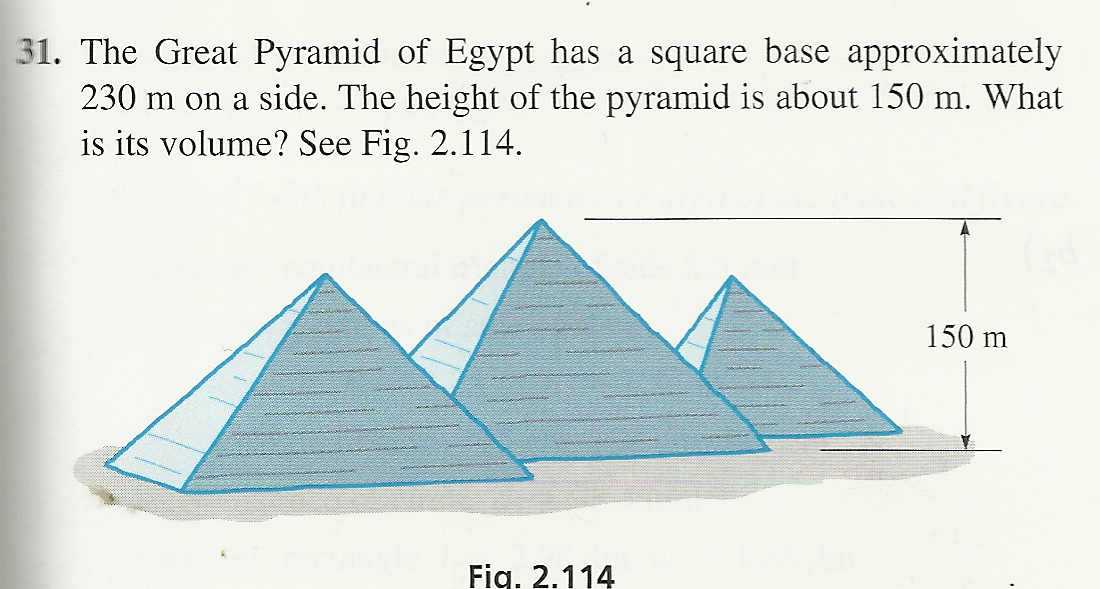
\includegraphics[scale=1]{./volume1.png}
  \end{figure}
\end{frame}

\begin{frame}
  \frametitle{Volume: Word Problems II}
  \begin{figure}[h]
    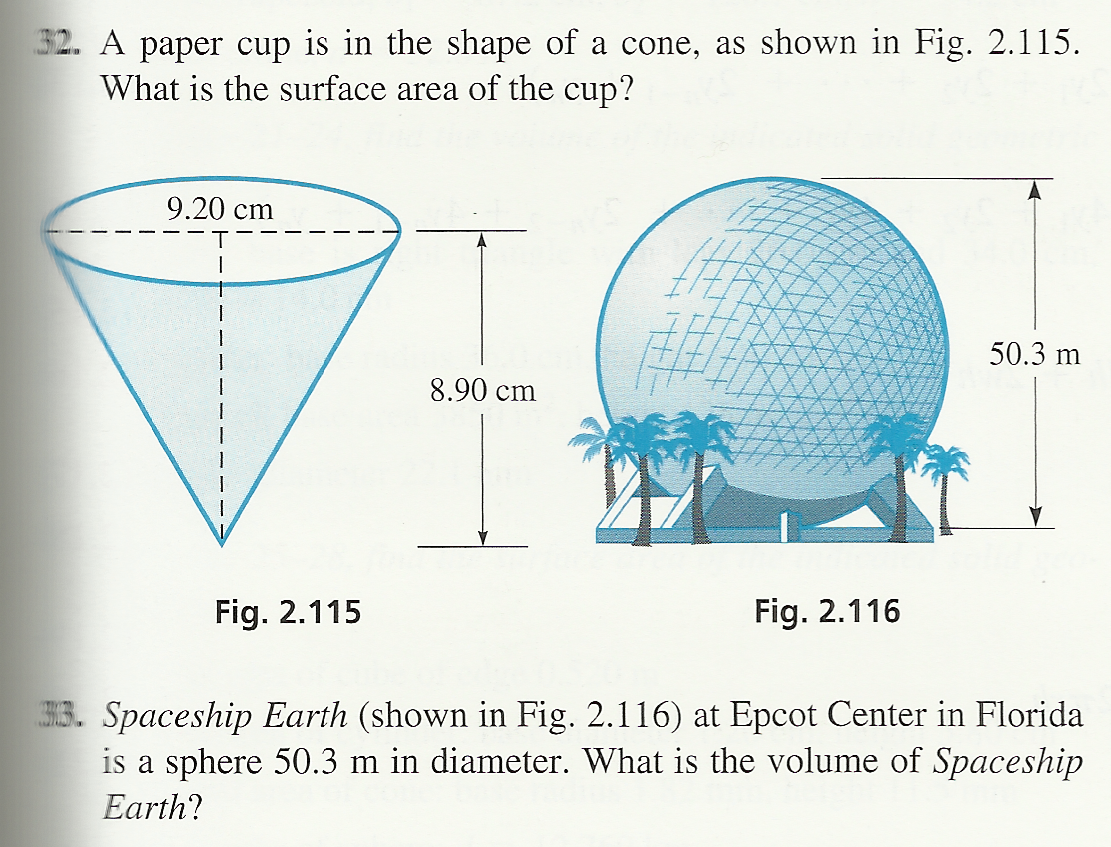
\includegraphics[scale=1]{./volume2.png}
  \end{figure}
\end{frame}

\begin{frame}
  \frametitle{Volume: Word Problems III}
  \begin{figure}[h]
    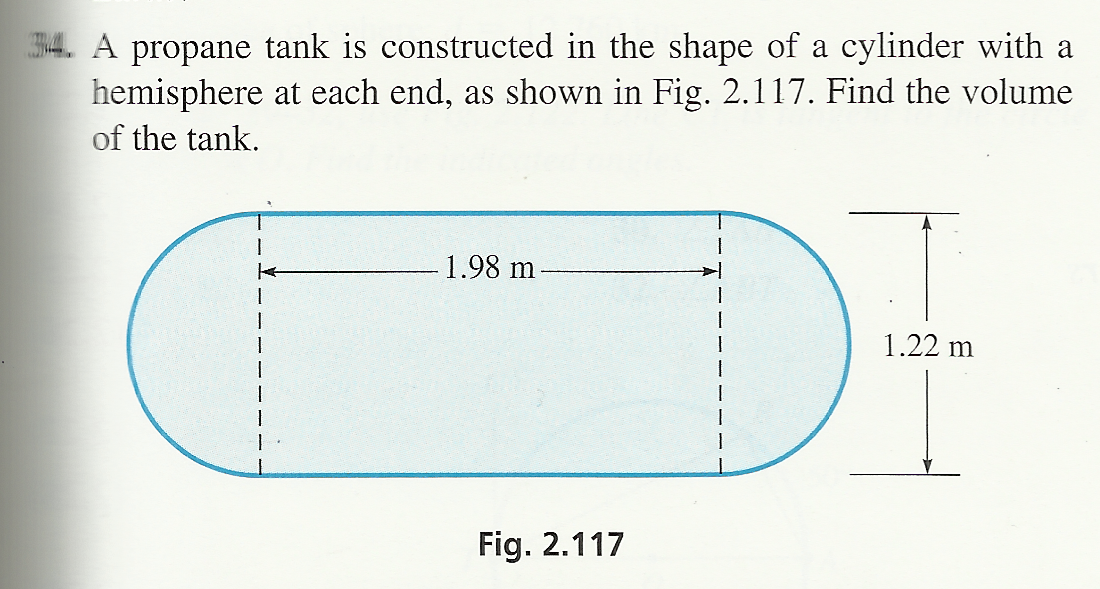
\includegraphics[scale=1]{./volume3.png}
  \end{figure}
\end{frame}

\begin{frame}
  \frametitle{End of Lesson}
Next Lesson: Normal Distribution.
\end{frame}

\end{document}
